\subsection{TCGA-BRCA results and ablation}
\label{sec:uni}
Among fourteen evaluated methods (Table~\ref{tab:uni_compare}), JPathGene
achieves the highest multimodal AUC and matches gene-only
($0.954$ vs.\ $0.954$; n.s.), while substantially reducing ECE relative to
gene-only ($0.094$ vs.\ $0.229$, $p\!<\!0.001$). This benefit is feature-dependent: with generic $2048$-dimensional ResNet-50
features the ordering reverses -- simple early and gated fusion lead (AUC $0.94$)
while JPathGene and gene-only trail ($\approx\!0.91$) -- and only with UNI2-h does
cross-modal learning reach the top. On pooled BRCA out-of-fold predictions,
JPathGene changes $26\%$ of gene-only decisions at the $0.5$ threshold and shifts
predicted probabilities by more than $0.10$ for $82\%$ of patients. Full has
lower F1 because its conservative probabilities reduce recall at the fixed
$0.5$ threshold, whereas CoRE recovers F1 through the gene anchor at the cost
of higher ECE. The variants therefore trade calibration against thresholded
classification performance.

\begin{table}[t]
\centering
\caption{TCGA-BRCA comparison using UNI2-h features and leakage-safe
5-fold$\times$5-seed CV (mean$\pm$std). Best AUC and ECE are bold.}
\label{tab:uni_compare}
\begin{tabular}{lccc}
\toprule
Method & AUC\,$\uparrow$ & F1\,$\uparrow$ & ECE\,$\downarrow$ \\
\midrule
\multicolumn{4}{l}{\emph{Unimodal}}\\
Gene-only & \textbf{0.954\,$\pm$\,0.018} & 0.748\,$\pm$\,0.066 & 0.229\,$\pm$\,0.024 \\
Image-only & 0.775\,$\pm$\,0.025 & 0.367\,$\pm$\,0.210 & 0.104\,$\pm$\,0.010 \\
\midrule
\multicolumn{4}{l}{\emph{Multimodal fusion baselines}}\\
Concat fusion & 0.928\,$\pm$\,0.033 & 0.392\,$\pm$\,0.127 & 0.088\,$\pm$\,0.027 \\
Contrastive (CLIP-style) & 0.927\,$\pm$\,0.052 & 0.436\,$\pm$\,0.203 & 0.081\,$\pm$\,0.023 \\
Late fusion & 0.917\,$\pm$\,0.037 & 0.534\,$\pm$\,0.165 & 0.079\,$\pm$\,0.022 \\
Early fusion & 0.915\,$\pm$\,0.044 & 0.683\,$\pm$\,0.080 & 0.099\,$\pm$\,0.029 \\
Cross-attention & 0.910\,$\pm$\,0.037 & 0.470\,$\pm$\,0.109 & 0.078\,$\pm$\,0.014 \\
Gated fusion & 0.890\,$\pm$\,0.042 & 0.515\,$\pm$\,0.093 & 0.087\,$\pm$\,0.017 \\
TabTransformer concat & 0.807\,$\pm$\,0.024 & 0.497\,$\pm$\,0.062 & 0.119\,$\pm$\,0.027 \\
\midrule
\multicolumn{4}{l}{\emph{JPathGene (ours)}}\\
\textbf{Full} & \textbf{0.954\,$\pm$\,0.010} & 0.602\,$\pm$\,0.122 & 0.094\,$\pm$\,0.033 \\
\textbf{CoRE} & 0.953\,$\pm$\,0.016 & 0.743\,$\pm$\,0.034 & 0.190\,$\pm$\,0.039 \\
\textbf{MLP predictor} & 0.941\,$\pm$\,0.022 & 0.466\,$\pm$\,0.125 & 0.080\,$\pm$\,0.021 \\
\textbf{Diffusion (PCA)} & 0.916\,$\pm$\,0.046 & 0.593\,$\pm$\,0.132 & \textbf{0.071\,$\pm$\,0.020} \\
\textbf{Full (diff.+pathway)} & 0.882\,$\pm$\,0.041 & 0.495\,$\pm$\,0.110 & 0.076\,$\pm$\,0.013 \\
\bottomrule
\end{tabular}
\end{table}

\paragraph{Calibration.}
\label{sec:calib}
Because ECE is binning-sensitive, we additionally report Brier score and NLL
(Table~\ref{tab:calibration}). JPathGene attains the lowest Brier score ($0.089$)
and NLL ($0.276$), compared with $0.147$ and $0.463$ for gene-only, indicating
better probabilistic predictions beyond bin-based calibration.

\begin{table}[t]
\centering
\caption{Proper scoring rules on pooled out-of-fold predictions
(mean$\pm$std over five seeds; lower is better). Best values are bold.}
\label{tab:calibration}
\begin{tabular}{lcc}
\toprule
Method & Brier & NLL \\
\midrule
Image-only & 0.140\,$\pm$\,0.007 & 0.495\,$\pm$\,0.029 \\
Gene-only & 0.147\,$\pm$\,0.059 & 0.463\,$\pm$\,0.141 \\
Concat fusion & 0.102\,$\pm$\,0.014 & 0.322\,$\pm$\,0.041 \\
\textbf{JPathGene (ours)} & \textbf{0.089\,$\pm$\,0.014} & \textbf{0.276\,$\pm$\,0.033} \\
\bottomrule
\end{tabular}
\end{table}

\paragraph{Ablation.}
A $2^4$ factorial ablation identifies the gene anchor as the dominant component,
with anchored configurations reaching AUC $0.94$--$0.96$ versus
$0.84$--$0.92$ without it. Masked and cross-modal JEPA reduce variance,
whereas contrastive alignment adds little benefit.

\subsection{TCGA-LUAD validation}
\label{sec:luad}
We further evaluate JPathGene on TCGA-LUAD
(Table~\ref{tab:luad_combined}). For TP53 mutation, CoRE significantly
outperforms gene-only in both AUC ($0.793$ vs.\ $0.774$, $p\!=\!0.028$)
and calibration ($p\!=\!0.041$). For stage classification, all multimodal
methods improve AUC by $0.07$--$0.11$ over gene-only ($p\!<\!0.001$),
indicating complementary histologic information. The gate therefore adjusts
the image contribution according to cross-modal reliability.
Figure~\ref{fig:qualitative} shows held-out cases recovered by JPathGene when
the unimodal and concatenation models fail.

\begin{table}[t]
\centering
\caption{TCGA-LUAD validation using UNI2-h features and
5-fold$\times$5-seed CV (mean$\pm$std).
Best AUC and ECE per endpoint are bold.}
\label{tab:luad_combined}
\resizebox{\linewidth}{!}{%
\begin{tabular}{lcccc}
\toprule
& \multicolumn{2}{c}{TP53 mutation ($n{=}460$)} & \multicolumn{2}{c}{Stage early/II$+$ ($n{=}393$)} \\
\cmidrule(lr){2-3}\cmidrule(lr){4-5}
Method & AUC & ECE & AUC & ECE \\
\midrule
Image-only & 0.693\,$\pm$\,0.013 & 0.237\,$\pm$\,0.044 & 0.662\,$\pm$\,0.032 & 0.224\,$\pm$\,0.023 \\
Gene-only & 0.774\,$\pm$\,0.006 & 0.181\,$\pm$\,0.041 & 0.578\,$\pm$\,0.014 & \textbf{0.166\,$\pm$\,0.031} \\
Concat fusion & 0.764\,$\pm$\,0.012 & 0.202\,$\pm$\,0.042 & 0.650\,$\pm$\,0.017 & 0.230\,$\pm$\,0.029 \\
Late fusion & 0.745\,$\pm$\,0.013 & 0.209\,$\pm$\,0.027 & \textbf{0.684\,$\pm$\,0.019} & 0.209\,$\pm$\,0.033 \\
\textbf{JPathGene (full, ours)} & 0.769\,$\pm$\,0.019 & 0.195\,$\pm$\,0.025 & 0.661\,$\pm$\,0.013 & 0.227\,$\pm$\,0.042 \\
\textbf{JPathGene (gene-anchored, ours)} & 0.770\,$\pm$\,0.017 & 0.183\,$\pm$\,0.041 & 0.669\,$\pm$\,0.012 & 0.188\,$\pm$\,0.039 \\
\textbf{JPathGene (CoRE, ours)} & \textbf{0.793\,$\pm$\,0.012} & \textbf{0.118\,$\pm$\,0.028} & 0.669\,$\pm$\,0.011 & 0.223\,$\pm$\,0.026 \\
\bottomrule
\end{tabular}%
}
\end{table}


\begin{figure}[!htb]
    \centering
    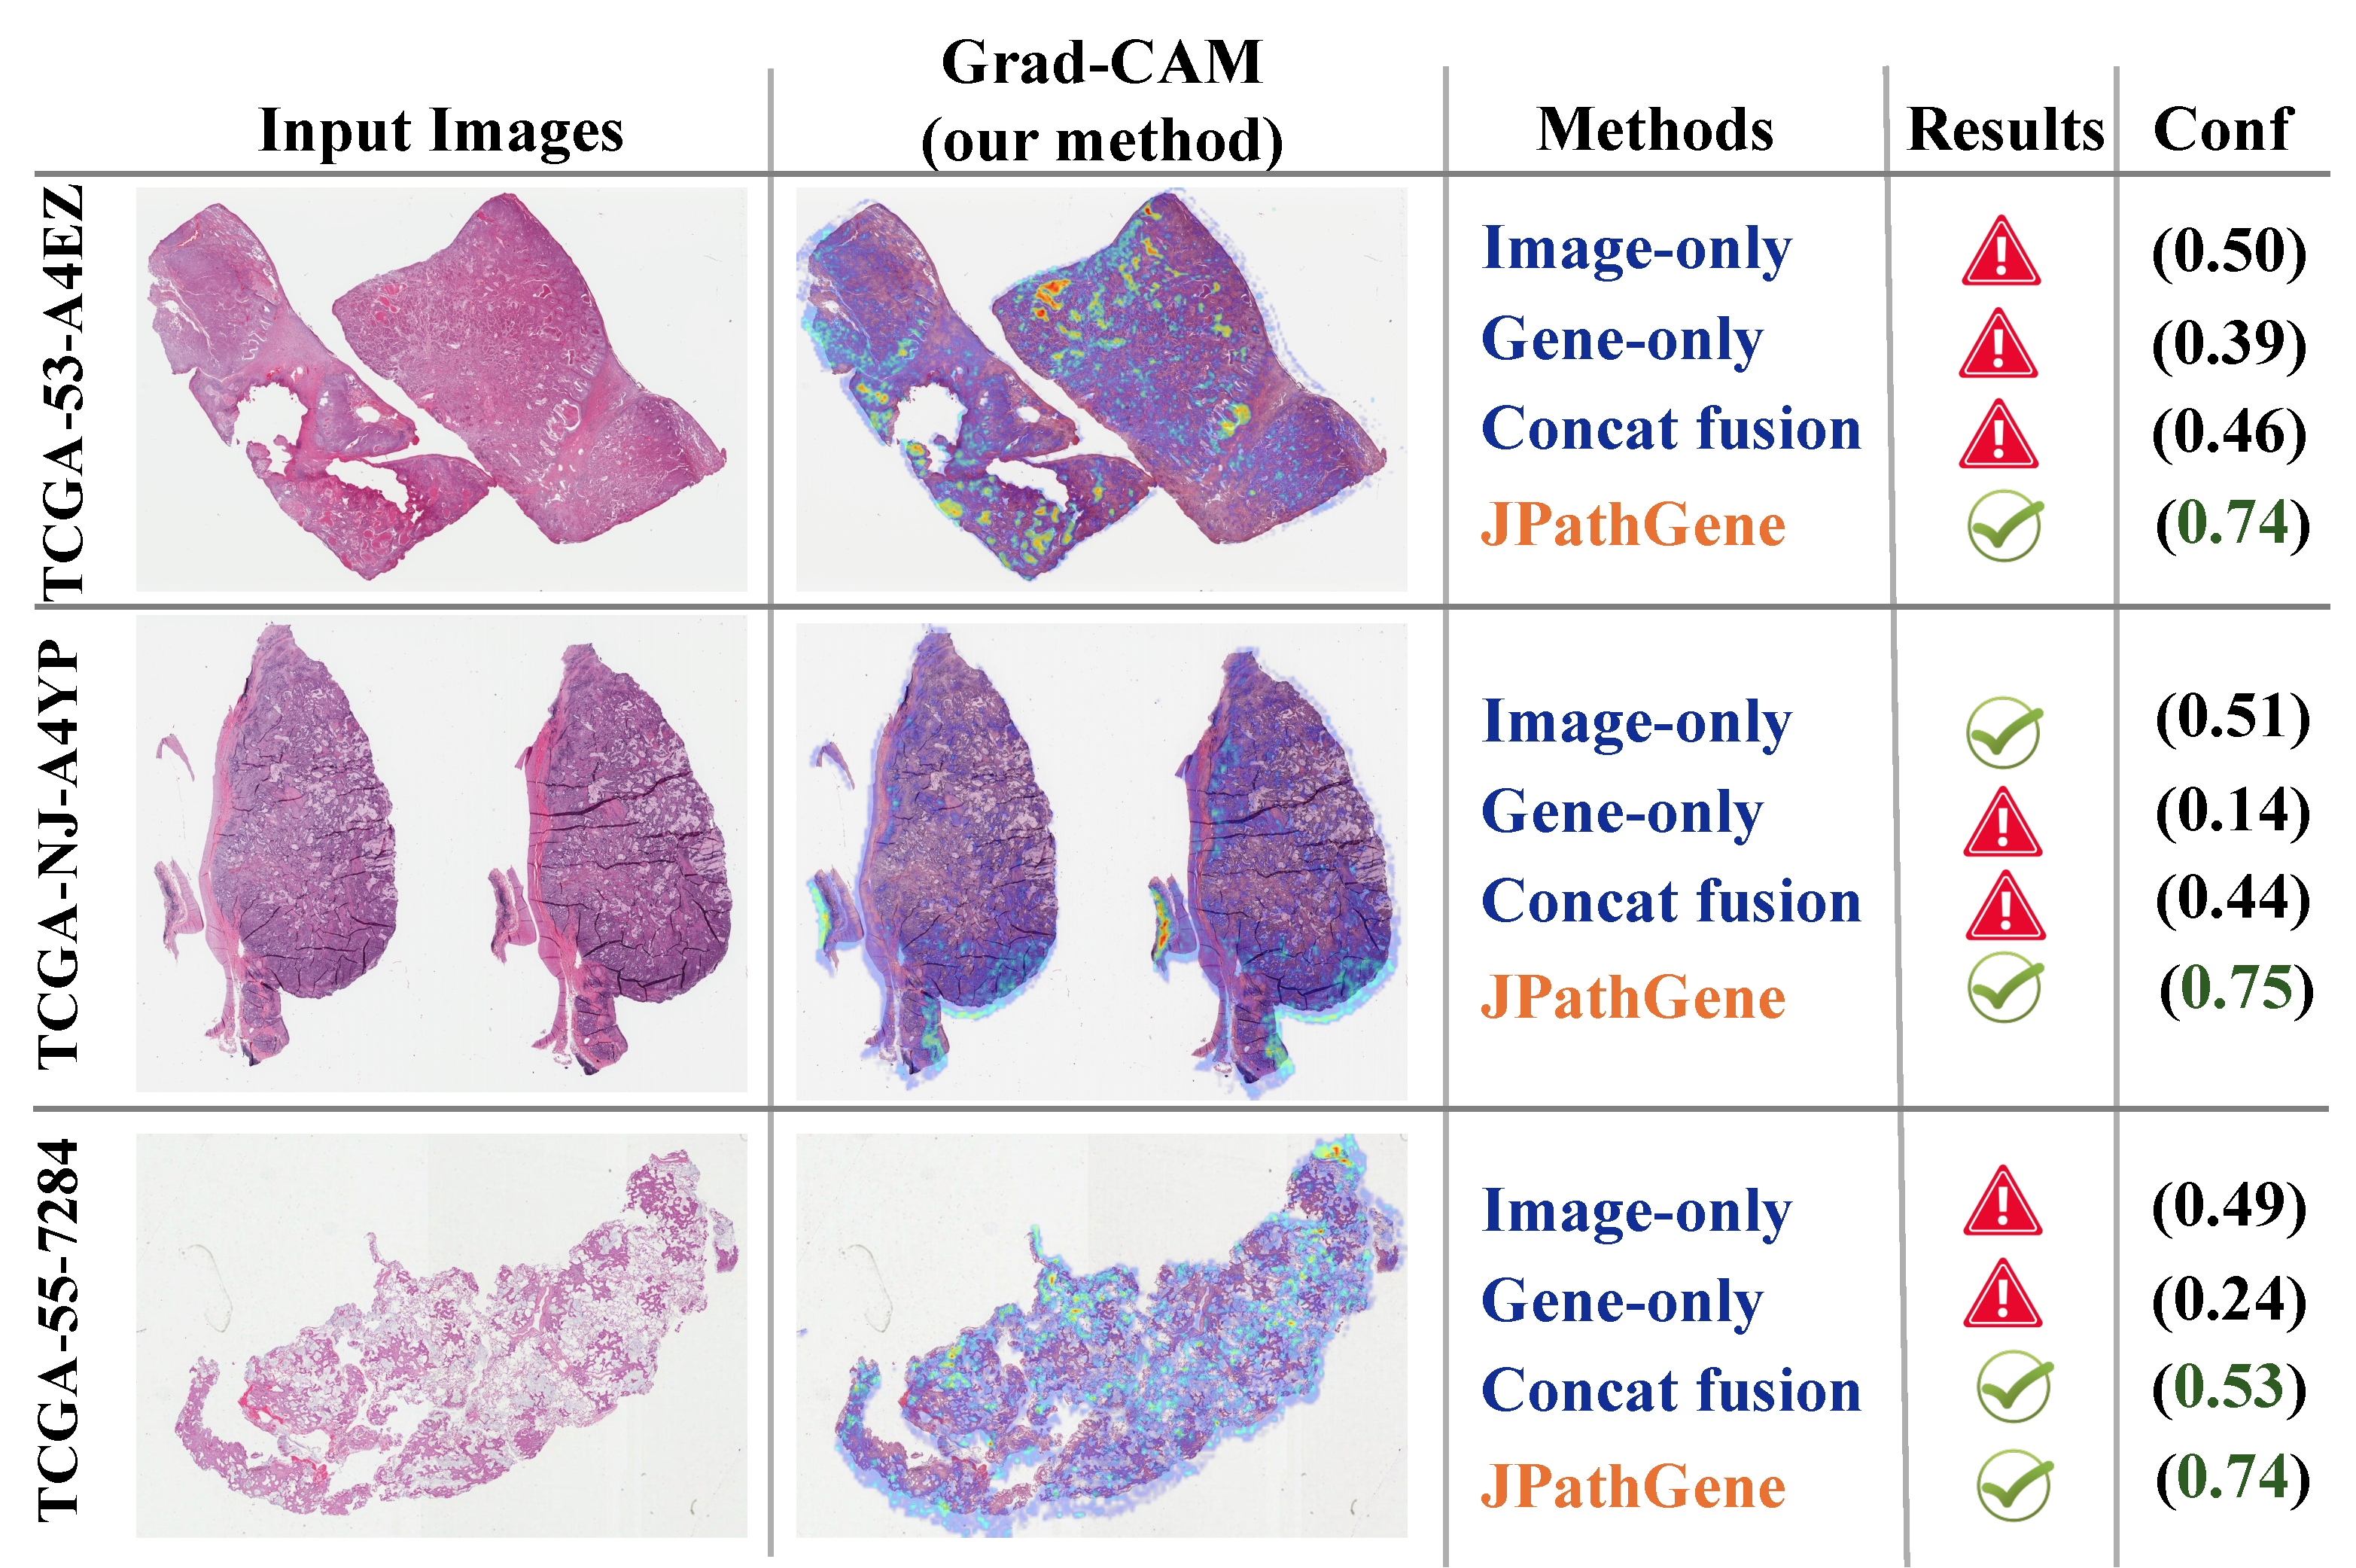
\includegraphics[width=0.8\linewidth]{figures/fig3.pdf}
    \caption{\textbf{LUAD-stage examples.} JPathGene correctly classifies
held-out cases missed by image-only, gene-only, and concatenation fusion.}
    \label{fig:qualitative}
\end{figure}
